\chapter{Manual de Usuario para las Familias}
\label{chap:manfamilias}

A continuación, se detallará el uso de la aplicación móvil, así como las funcionalidades principales para los usuarios de las familias registradas.

\subsection*{Iniciar Sesión}
La primera vez que se ejecuta la aplicación se debe iniciar sesión usando número de teléfono o correo electrónico y contraseña, métodos que se encuentran disponibles mediante dos botones en la pantalla inicial (Figura \ref{fig:inicioappfamilia}), reservándose el último botón <<Soy Docente>> para los docentes del centro.

\begin{figure}[!h]
	\begin{center}
		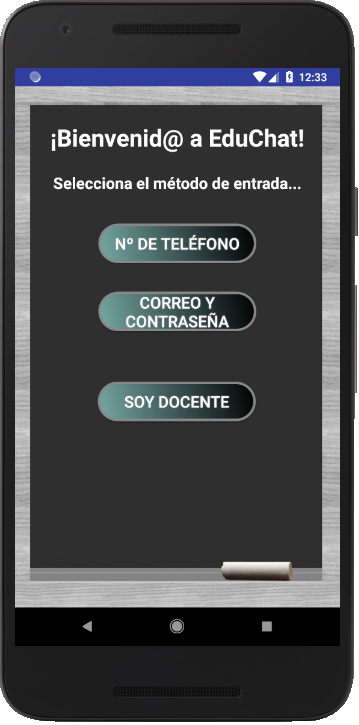
\includegraphics[width=0.35\textwidth]{/manuales/familia/inicioapp}
		\caption{Pantalla Inicio de la Aplicación}
		\label{fig:inicioappfamilia}
	\end{center}
\end{figure}

\clearpage

Si se selecciona iniciar sesión mediante número de teléfono, se deberá introducir este en la aplicación y pulsar el botón <<Enviar Código>> (Figura \ref{fig:iniciotfnofamilia}). Acto seguido, se recibirá en el terminal un mensaje \acs{SMS} con un código que se deberá introducir para completar el inicio de sesión. Por el contrario, si se selecciona el método de entrada mediante correo y contraseña, se deberán introducir ambos parámetros y pulsar el botón <<Enviar>> (Figura \ref{fig:iniciocorreofamilia}). Si es la primera vez que se inicia sesión en la aplicación, la contraseña que se introduzca en el campo correspondiente será la que se use para futuros inicios de sesión. No obstante, esta contraseña se puede cambiar haciendo uso de la opción <<¿Has olvidado tu contraseña?>>. En este caso, se deberá introducir el correo electrónico al que se desea que se mande el mensaje de recuperación con las instrucciones necesarias. Principalmente, este mensaje consta de un enlace que se deberá seguir para introducir la nueva contraseña.

\begin{figure}[!h]
	\centering
	\begin{minipage}{.5\textwidth}
		\centering
		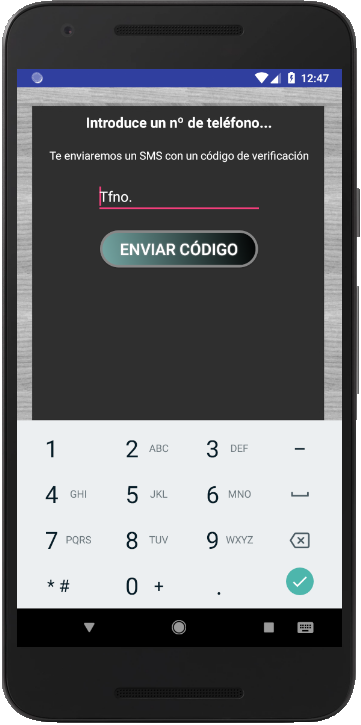
\includegraphics[width=0.6\textwidth]{/manuales/familia/iniciotfno}
		\caption{Pantalla de Inicio de Sesión \\ Mediante Nº de Teléfono}
		\label{fig:iniciotfnofamilia}
	\end{minipage}%
	\begin{minipage}{.5\textwidth}
		\centering
		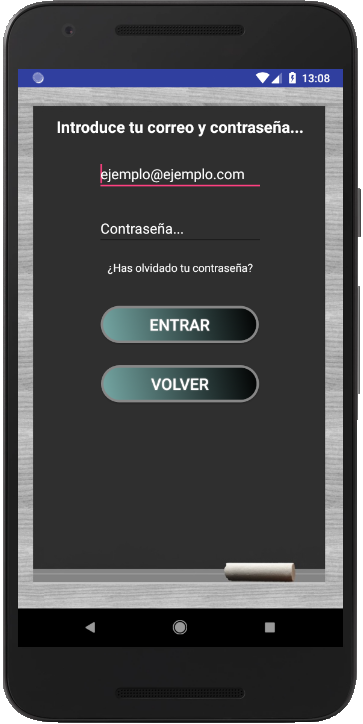
\includegraphics[width=0.6\textwidth]{manuales/familia/iniciocorreo}
		\caption{Pantalla de Inicio de Sesión \\ Mediante Correo y Contraseña}
		\label{fig:iniciocorreofamilia}
	\end{minipage}
\end{figure}

\clearpage

\subsection*{Ver y Editar Perfil}
Una vez que se ha accedido a la aplicación, se puede visualizar la información registrada acerca de la familia. Para ello, se debe pulsar la opción <<Perfil...>>, situada en el menú principal de la aplicación que se encuentra en la esquina superior derecha, representado por tres puntos en posición vertical. Una vez dentro, se podrá, además, establecer una imagen personalizada para la familia o eliminarla y restablecer la imagen por defecto usando los botones <<Cambiar Imagen de Perfil>> y <<Eliminar Imagen de Perfil>>, respectivamente (Figura \ref{fig:perfilfamilia}).

\begin{figure}[!h]
	\begin{center}
		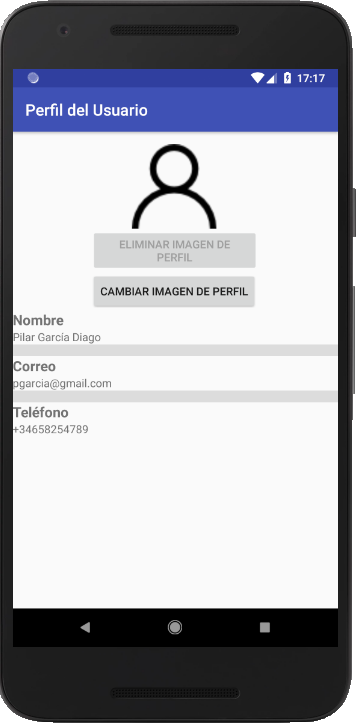
\includegraphics[width=0.4\textwidth]{/manuales/familia/perfil}
		\caption{Pantalla de Perfil}
		\label{fig:perfilfamilia}
	\end{center}
\end{figure}

\clearpage

\subsection*{Ver y Enviar Mensajes}
Los usuarios de las familias podrán ver los chats a los que han sido añadidos, no pudiendo crear nuevos. Todos estos chats se mostrarán en la pantalla principal de la aplicación en forma de lista y, pulsando sobre cada uno de ellos, entrarán a los mismos y podrán enviar y recibir mensajes.

\subsection*{Ver Información del Chat}
Los usuarios de la aplicación tienen disponible un botón <<Info.>> en cada chat, desde donde se puede ver el nombre del grupo, así como las familias que lo integran (Figura \ref{fig:infochatfamilia}).

\begin{figure}[!h]
	\begin{center}
		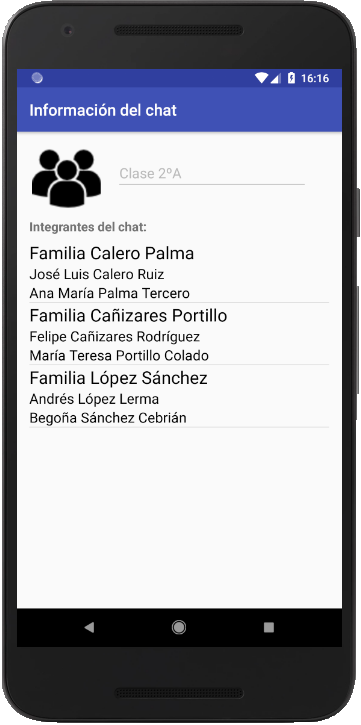
\includegraphics[width=0.4\textwidth]{/manuales/familia/infogrupo}
		\caption{Pantalla de Información de Chat}
		\label{fig:infochatfamilia}
	\end{center}
\end{figure}